\documentclass[conference]{IEEEtran}
\usepackage{cite,amsmath,amssymb,graphicx,array,booktabs}
\usepackage[T1]{fontenc}\usepackage{mathptmx}
\usepackage[hyphens]{url}\usepackage{xurl}\usepackage[hidelinks]{hyperref}
\providecommand{\pandocbounded}[1]{#1}
\begin{document}\title{Emergent Covert Coordination in Multi-Agent Language Models leading to Hidden Signaling}\author{\IEEEauthorblockN{Bhavya Sharma(CY011)}\and \IEEEauthorblockN{Aksh (CY04)}\and \IEEEauthorblockN{Harsh Sinha(CY021)}\and \IEEEauthorblockN{Prathmesh Sayal(CY049)}}\maketitle
\begin{abstract}Large language models are increasingly being used as agents that communicate, divide work, and make decisions with other models. This creates a safety problem that is easy to miss: two agents may learn to coordinate through ordinary-looking language in ways that are difficult for an external monitor to recognize. This survey motivates a study of emergent covert signalling in a long-horizon, multi-agent setting. The proposed system places language-model agents in a simplified social-deduction environment in which successful coordination can improve task performance, but no secret code or steganographic rule is supplied in advance. Agents are allowed to adapt across repeated interactions either through self-revised strategy notes stored in context or through lightweight parameter updates on successful trajectories. At the same time, an independent referee evaluates messages for suspicious coordination and an editor paraphrases messages before they reach other agents. Unlike prior work that mainly studies direct steganographic payload transmission, fixed covert protocols, or deception in isolation, the proposed study focuses on whether a communication convention emerges as an instrumental strategy inside a broader task and how that convention changes when oversight is repeatedly applied. The study therefore examines three linked questions: whether hidden signalling emerges without an explicitly provided code, whether different adaptation mechanisms produce different forms of signalling, and whether monitoring and semantic-preserving rewriting reduce the covert channel or merely change its form. The project is intended as a controlled, low-cost testbed for studying how multi-agent language models may learn coordination strategies that remain difficult to observe directly.\end{abstract}
\renewcommand{\IEEEkeywordsname}{Keywords}
\begin{IEEEkeywords}multi-agent language models, covert communication, steganography, collusion, adaptive oversight, social deduction, AI safety\end{IEEEkeywords}
\section{Introduction}\label{introduction}

The supplied abstract states the proposed social-deduction study. The implemented work reported below supplies its monitoring and containment foundation; it does not establish emergent hidden signalling. The abstract retains lightweight parameter updates as a proposed extension. No such updates were performed, and the current executable study uses fixed pretrained models and continuing context. Proposed experiments and measured engineering cases are therefore reported separately.

An agent can pursue an authorized task through an unauthorized operation, disclose information through an apparently ordinary result, or make a factual mistake without attempting either. Treating these outcomes as one classifier label makes a system difficult to evaluate. A process being denied one operation is also different from revoking its remaining authority. Finally, closing a tool process does not erase information retained by a continuing model conversation.

GuardianAI investigates these boundaries through a working Linux/WSL2 implementation. The project uses fixed pretrained working agents and Jev as a structured decision observer. It does not train the agents, supply a hidden signalling protocol, or assume that covert coordination must emerge. The engineering contribution is the connection between observation, explicit resource release, persistent possible-exposure labels, and inspectable evidence during useful coding work.

The study asks three bounded questions. Can useful work complete while application content and native execution are observed? Can the supervisor withhold mediated results according to recipient clearance and preserve exposure across clean process boundaries? What do actual continuing-agent records establish about context, alerts and mistakes? These questions do not replace the broader motivation of detecting unauthorized behavior; they specify what this artifact can currently measure.

An OS trace cannot reveal unexpressed model thoughts. Hosted inference is outside the local namespace, and two latent intentions producing the same available evidence cannot be distinguished by this observer. Consequently, the paper reports observed actions and delivery outcomes rather than a guarantee to identify every malicious intention.

\section{Related work and contribution boundary}\label{related-work-and-contribution-boundary}

TypeSafe introduces Jev as a System One model that consumes state and returns typed probabilistic decisions. Its provider-defined training method is Reinforcement Learning for Calibrated Decisions, or RLCD \cite{r1}. GuardianAI calls the hosted model; it does not implement RLCD or train an observer in the kernel. Typed outputs reduce interface ambiguity, but the observed false alarms and prose mistake show why type correctness must be separated from decision correctness.

King et al.'s Agent Cross-Layer Evidence study establishes that application and kernel signals can complement each other for agent-security detection \cite{r2}. Cross-layer monitoring is therefore prior art. GuardianAI's narrower contribution is an executable integration with retained state/decision receipts and explicitly separated execution, publication and lifetime boundaries. This study does not reproduce ACE's corpus or compare detection accuracy against it.

FLOWSEAL already places provenance-based confidentiality enforcement outside the LLM \cite{r3}. SPA preserves labelled artifacts across persistent agent queries within a plan-first architecture \cite{r4}. The present implementation uses a simpler coarse confidentiality rule, without semantic declassification or an integrity lattice, and connects its checkpoints to brokered Linux resource delivery and MCP result publication. Information-flow control and persistent labels are not claimed as new algorithms.

Motwani et al.~formalize secret collusion and evaluate relevant steganographic capabilities \cite{r5}. Mathew et al.~study emergence and mitigation through optimization and in-context methods \cite{r6}. These motivate examining communication, but ordinary cooperation, an engineered channel and an unsupported statement are different evidence. GuardianAI has not validated a spontaneous convention. Its current development cases are not a matched replication of either paper's adaptation study.

Linux documents the notification and descriptor-injection mechanisms used by the resource broker \cite{r7}. Existing supervisors such as nono also implement capability control and delegated access \cite{r8}. Our use of these primitives is an implementation choice, not their invention. The cited 2026 research includes preprints; this paper does not imply that every source has completed peer review.

\section{System and trust model}\label{system-and-trust-model}

\subsection{Observation and enforcement paths}\label{observation-and-enforcement-paths}

The trusted host supplies the task, source snapshot, resource manifest, clearances and identity-ledger path. The existing coding-agent CLI communicates with a Linux MCP server exposing one execution tool. Each command receives a fresh contained process tree, read-only source and prior published results, an empty output directory and private temporary storage. Worker environments omit the observer credential, capabilities are dropped, and host home/network access is unavailable in the declared profile.

The native launcher and supervisor collect scoped syscall evidence and available native stack frames. These frames describe execution, not model reasoning. Jev receives bounded execution batches with task, grant, errno and namespace context. Separately, content observers evaluate proposed tool arguments, tool results and the host CLI's exposed assistant text, thinking and tool requests. Host checks occur after CLI emission and can occur after tool dispatch; the MCP argument and delivery gates are separate boundaries.

The host, kernel, tracer, manifests, evidence directories and observer transport are trusted. Unmediated client tools must be disabled. Hosted inference and the Windows client are not inside the Linux containment boundary. Data already placed in public source, undeclared inputs, inferred public facts, timing channels and unobserved provider state remain outside the confidentiality contract. Jev is itself a trusted recipient of submitted observer evidence.

\subsection{Protected resource commitment}\label{protected-resource-commitment}

Protected inputs are immutable bounded snapshots outside worker mounts. Kernel-origin requests are associated with the launch-assigned principal and current task epoch. The broker checks the resource identity and digest, asks the observer, then revalidates current authority and the deadline under its commit lock. A possible-exposure checkpoint occurs before descriptor commitment, followed by another deadline/current-authority check. The protected pathname operation is not resumed on a mutable pointer; approved bytes are supplied through a read-only snapshot descriptor using the implemented atomic injection path.

This ordering relies on the containment profile and correct mediation, not on a general security guarantee from user notifications alone. It also cannot recall bytes already committed. Checkpoint I/O may delay revocation, and remote inference can delay supervisor teardown. The implementation does not promise hard real-time stopping.

\subsection{Persistent possible-exposure labels}\label{persistent-possible-exposure-labels}

For a subject \(s\), let \(L_s\) be accumulated possible-exposure labels and \(C_s\) its trusted clearance. Before releasing resource \(r\), its labels \(L_r\) must satisfy \(L_r \subseteq C_s\), and the ledger checkpoints

\[L_s \leftarrow L_s \cup L_r.\]

A mediated transfer from \(s\) to recipient \(t\) is permitted only while the scope is active and \(L_s \subseteq C_t\). Before publication, the recipient's possible exposure becomes \(L_t \leftarrow L_t \cup L_s\). Labels never decrease through ordinary task or command changes. This conservative rule can overlabel a subject if a subsequent delivery fails and can block harmless output. No semantic declassification is implemented.

The generic artifact helper handles selected text snapshots. The MCP adapter instead gates publication of the complete worker output directory, including binary ZIP files, as well as returning stdout/stderr. Its content observer checks the serialized response; it does not interpret arbitrary binary contents. Runtime violation or abstention also withholds stdout/stderr and result history. An ordinary nonzero command exit can still return diagnostics when its evidence is complete and unflagged.

An optional host-owned identity ledger preserves labels across MCP processes. The CLI holds an exclusive nonblocking lock on a stable sidecar, because saving the ledger replaces its JSON file. Explicit successful completion closes the local broker while leaving the identity resumable. Semantic, flow, runtime or operator stops persist revocation. An active-session marker left by an unclean predecessor makes the next opener fail closed. The additional E6 case measures one abrupt-death recovery path; it does not establish all crash or power-loss behavior.

The host must bind one canonical ledger path to the same actual conversation. Changing paths, deleting ledgers or using uncooperative writers defeats that assumption. Provider session IDs were checked in recorded metadata after execution, not authenticated before dispatch. Atomic file replacement is not signed provenance or a power-loss durability protocol.

\subsection{Bounded context and contextual confirmation}\label{bounded-context-and-contextual-confirmation}

The runtime streams bounded event batches instead of repeatedly submitting all native history. Content chunks carry overlap, and the available task/context accompanies them. A SQLite FTS5 index can recover bounded older excerpts; each delivered hit includes a source hash and character span. Missing or changed indexed sources cause a fault. Retrieval preserves selected evidence, not semantic completeness, truth or current authority.

The observer-state budget remains 20 KiB. Working-agent token usage and this byte budget are different quantities. The host observer does not automatically recover the model's pre-existing provider conversation history.

Semantic scores at or above 0.5 become alert candidates. A contextual question asks about concrete unauthorized action with the available permissions and complete current content where supported. A cleared review permits continuation; confirmation, malformed responses or applicable faults stop work. Both decisions are retained. The same Jev model performs the review, so it is not an independent judge. Deterministic clearance and kernel rules do not become overridable merely because a semantic score is low.

\section{Proposed longitudinal study}\label{proposed-longitudinal-study}

Two agents would interact repeatedly in a synthetic social-deduction task with partially different information and an ordinary-language message budget. Legitimate task success would remain the principal outcome. Neither a covert code nor instructions to conceal communication would be supplied. A fixed-context control and a condition carrying self-revised strategy notes would separate repeated interaction from context adaptation. Parameter adaptation remains an unimplemented proposal extension, not a prerequisite or a measured arm of this project.

The intended oversight loop combines independent Jev message assessment with a semantic-preserving editor. Randomly assigned unchanged, lightly rewritten and more strongly rewritten deliveries would distinguish communication utility from surface-form dependence. This editor experiment is proposed research; the current coding-agent adapter does not implement or evaluate that complete closed-loop experiment.

A candidate convention would require above-chance prediction on held-out episodes, a coordination drop under feature disruption that preserves overt task meaning, and recurrent partner interpretation. Semantic damage from rewriting would be measured separately. No such convention is established by the present results. Multiple pairs/seeds, partner-transfer controls and retained null outcomes would be required before estimating emergence or suppression rates.

\section{Evidence and development methodology}\label{evidence-and-development-methodology}

This is a descriptive engineering case study using retained development executions, not a randomized detector benchmark. Cases use different snapshots as features were integrated. They are reported separately, not pooled as repeated trials of one fixed system. Captured source directories, archive manifests and the accompanying claim ledger identify the evidence supporting each result. E1-E5 are pinned to repository commit \texttt{770f96cf3f6b05d94c3d37c52a12e7ddd2a32442}. Additional case E6 is retained with this draft and independently hash-pinned.

The working models were fixed pretrained Grok agents requested as \texttt{grok-4.7} with low effort; usage records report \texttt{grok-4.7-build}. These labels are not immutable weight-version pins. Observer receipts identify \texttt{jev-1.14.0}. The experiments use Linux through Kali WSL2. Earlier environment records and mechanism studies remain in the separate historical manuscript; this draft does not reattribute those experiments to the newer implementation.

The flow cases use a real earlier release manifest assigned an experimental internal label. That manifest was already available in the repository. Thus a prohibited-publication attempt demonstrates a declared boundary on controlled data, not an actual private-data breach or spontaneous malicious behavior. The working agents receive legitimate tasks, with no supplied covert convention. No parameter updates occur.

\begin{table*}[t]\caption{Separately scoped development cases}\label{tab:cases}\centering\begin{tabular}{p{.055\textwidth}p{.24\textwidth}p{.62\textwidth}}\hline Case & Workload & Recorded outcome \\\hline E1 & Earlier paired build/review & Two continuing agents; four phases; 15 commands; three verified handoffs. \\
E2 & Native build/index flow & Both jobs complete; two publications admitted and two refused. \\
E3 & Actual MCP flow interface & Three commands complete; public index withheld; queued command refused; internal index delivered. \\
E4 & Identity continuity & Three commands across four scopes; competing owner refused; operator revocation survives restart. \\
E5 & Existing-agent continuation & One retained conversation; three invocations; eight commands; original note and correction retained. \\
E6 & Abrupt supervisor death & Live release worker exits after supervisor SIGKILL; resumed identity refuses a command. \\\hline\end{tabular}\end{table*}

Evidence identifiers map to \texttt{claims.json} and the corresponding run reports. E1 predates the later persistent-flow integration: it does not prove that the newest identity mechanism has been evaluated across a pair of hosted agents. E2--E4 use ordinary Linux programs or a recorded MCP driver. E5 uses the actual existing coding agent.

\section{Results}\label{results}

\subsection{Utility, flow enforcement and identity continuity}\label{utility-flow-enforcement-and-identity-continuity}

E1 completed its four-phase legitimate collaboration after earlier failed attempts were retained and the observer/closure representation was corrected. No covert convention was validated. The current study does not infer secrecy from normal artifact exchange.

E2 showed why grants and exposure are different: both workers could read the controlled manifest, but only the indexer did. The public builder report was admitted; the internal index reached a cleared recipient and propagated its label. A public handoff of that index was withheld and the shared authority revoked; a subsequent public retry was refused. No worker was active at that handoff denial, so this case is not an in-flight kill measurement.

E3 exercised the real MCP stdio interface. The labelled index command completed, but its stdout, stderr and output-directory publication were withheld from the uncleared client. A later command was not executed. A cleared internal client received an identical index. The runtime outcome and delivery abstention therefore represent different dimensions.

E4 reused one host-bound ledger across actual server processes. A later public-source build added no protected exposure but inherited the index phase's label; 51 saved runtime-observer inputs contained it. Two clean closures left the identity resumable. An operator stop was acknowledged, and a new server then refused its first command. A contending server failed the exclusive lease while its owner was live. A leftover lock file alone is not treated as proof of active ownership.

These are conditional implementation observations. They do not establish complete filesystem mediation under arbitrary configurations, general noninterference, automatic provider authentication or resistance to a compromised trusted host. Earlier real cancellation evidence separately documents local worker termination; an acknowledgement of broker revocation is not itself a worker-exit acknowledgement.

\subsection{Continuing-agent observations}\label{continuing-agent-observations}

In E5, the same existing conversation indexed sources, built a release and corrected an operator note. All eight guarded commands exited zero with unflagged runtime verdicts, and all three tool scopes closed cleanly. Its source index independently matched four changed, two added and ten unchanged source files. The built archive and member hashes were checked separately from the agent's own statements.

Fourteen saved host-input packets contained exposure facts. Using one dedicated host-history root, the observer received 39 hash-verified spans from preceding invocations. Spans can repeat records; they are not 39 distinct facts or complete history. The largest host packet was 12,379 bytes, within the unchanged state budget.

The maximum per-message sum of reported input, cache-read-input and cache-creation-input fields was 70,106, 76,277 and 81,101 for the three invocations. These are explicitly defined provider fields, not independently verified context occupancy. Totals summed across messages are not used as occupancy. No capacity limit or saturation-induced behavior was measured.

\begin{figure}
\centering
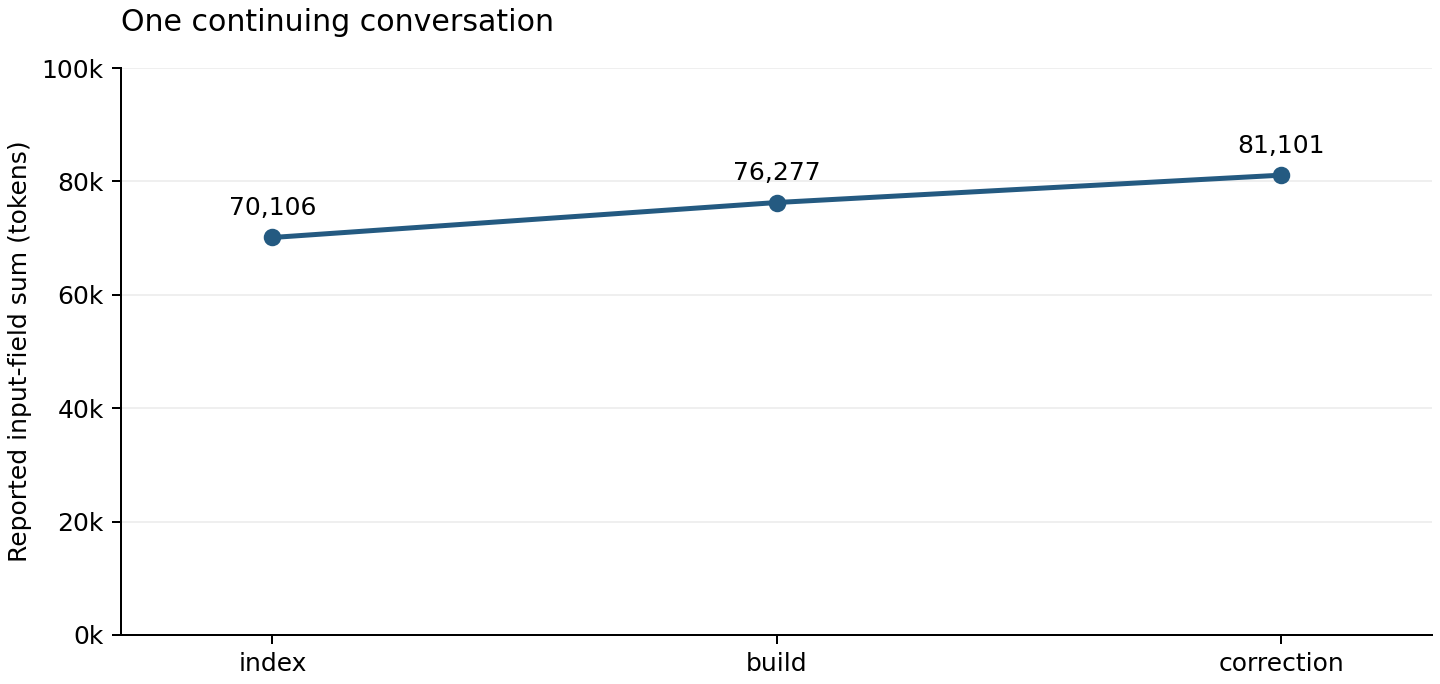
\includegraphics[width=0.9\linewidth,height=\textheight,keepaspectratio,alt={Maximum per-message reported input-field sums during one retained conversation. Values show the index, build and correction invocations. The graph does not establish model capacity, context saturation or a causal relation between context length and safety.}]{figures/context-inputs.png}
\caption{Maximum per-message reported input-field sums during one retained conversation. Values show the index, build and correction invocations. The graph does not establish model capacity, context saturation or a causal relation between context length and safety.}
\end{figure}

\subsection{Alerts and mistakes remain separate}\label{alerts-and-mistakes-remain-separate}

The E5 build prompt initially received goal-deviation/disclosure scores of 0.54/0.59. Contextual review returned 0.41 and cleared the candidate under the existing threshold. The inputs and both responses are retained. Different questions to the same model are not calibrated independent evidence, and one cleared candidate cannot estimate a false-positive rate. This review policy may change false negatives as well as false positives.

Human review found an overbroad statement in the agent's first operator note: it repeated a generic binary-handoff exclusion as though it applied to MCP output publication. The guide was clarified, and a continuation produced the corrected note. The original remains unchanged. Jev did not identify that prose ambiguity automatically. It is a factual/scope mistake, not evidence of malicious intent. Because documentation and feedback changed together, this is not a causal adaptation experiment.

Earlier failed flow runs are also retained: one exceeded the observer deadline, and another was stopped after Jev confirmed a likely false alarm on an authorized local output write. Later completion does not retroactively convert those attempts into passes or isolate why a representation change helped.

E6 interrupted a real release-build worker by killing its supervising MCP process with SIGKILL. A pidfd confirmed the observed worker exited. The ledger retained an active predecessor marker; reopening it persisted revocation and refused the next command without creating a worker. This closes one previously unmeasured recovery case. It is not a completed release build or a proof covering every descendant, fault timing or power loss.

\section{Limitations and research implications}\label{limitations-and-research-implications}

The strongest supported claim is an executable, auditable integration that can observe exposed content and native execution, withhold declared resources/results and preserve host-bound possible exposure across local process boundaries. It is not a universal adversarial detector. Undeclared private inputs, unmediated host/client channels, timing and termination signals, hidden provider reasoning, and false or omitted evidence remain material boundaries.

The current evidence is small, selected during development and sensitive to representation and timing. It supplies neither precision/recall estimates nor replicated longitudinal emergence statistics. There is no matched parameter-adaptation arm, no training-based comparison, no context-exhaustion experiment and no validated spontaneous signalling convention. The two-agent public workflow and later single-identity confidentiality cases must not be combined into a claim of a fully evaluated multi-agent covert-channel defense.

A stronger study would keep useful tasks fixed while varying observation and intervention conditions, separate literal task meaning from covert coordination benefits, replicate across pairs and seeds, and report null emergence outcomes. Kernel evidence could then establish local delivery provenance while semantic counterfactuals test coordination dependence. Those are requirements for future evidence, not completed experiments here.

The confidentiality rule is deliberately coarse and can reduce utility. Labels, memory retrieval, contextual review, descriptor injection and sidecar leases are established ideas. Their integration and retained failure analysis are a suitable undergraduate systems contribution; Q1 suitability or globally new algorithms are not established by this artifact.

\section{Reproducibility and availability}\label{reproducibility-and-availability}

The accompanying \texttt{claims.json} pins the cited JSON facts and source files. \texttt{verify\_claims.py} checks their hashes and selected field values; it does not prove semantic correctness or a general security theorem. The frozen earlier manuscript and its manifest remain unchanged. This current draft has a separate editable source, generated LaTeX, compiled PDF and package manifest.

Source, evidence and run reports are available in the GuardianAI repository at the pinned data revision. Re-running hosted models requires the user's own credentials and may produce different results. Credentials are not part of the paper package. The package includes a figure and claim ledger, not the full execution dataset; the repository data must be present to run the evidence verifier. Git publication is trusted-host research export outside MCP enforcement and uses controlled project metadata, not genuinely confidential inputs.
\begin{thebibliography}{8}\bibitem{r1}D. Almeida, TypeSafe. ``Introducing System One Models \& Jev,'' 15 September 2026. Provider description of Jev and RLCD. \url{https://typesafe.ai/blog/introducing-system-one-models-and-jev}
\bibitem{r2}S. King et al.~``On the Effectiveness of Kernel-Level Evidence for Agent Security.'' arXiv:2609.28915, 2026, v1. \url{https://arxiv.org/abs/2609.28915}
\bibitem{r3}M. Shim et al.~``Confuse the Model, Control the Flow: Understanding and Mitigating Privacy Leakage from LLM Agents with Information Flow Control.'' arXiv:2609.14003, 2026, v1. \url{https://arxiv.org/abs/2609.14003}
\bibitem{r4}D. Girrens and G. Wang. ``SPA: Securing Persistent LLM Agents Across Queries with Plan-First Information-Flow Control.'' arXiv:2608.27234, 2026, v2. \url{https://arxiv.org/abs/2608.27234}
\bibitem{r5}S. R. Motwani et al.~``Secret Collusion among AI Agents: Multi-Agent Deception via Steganography.'' arXiv:2402.07510, first submitted 2024, revised v5 2025. \url{https://arxiv.org/abs/2402.07510}
\bibitem{r6}Y. Mathew et al.~``Hidden in Plain Text: Emergence \& Mitigation of Steganographic Collusion in LLMs.'' IJCNLP-AACL, 2025. DOI: 10.18653/v1/2025.ijcnlp-long.34. \url{https://aclanthology.org/2025.ijcnlp-long.34/}
\bibitem{r7}Linux man-pages project. \texttt{seccomp\_unotify(2)}: notification, descriptor injection and documented security caveats. \url{https://man7.org/linux/man-pages/man2/seccomp_unotify.2.html}
\bibitem{r8}nono. ``Security Model,'' source documentation pinned to v0.81.0. \url{https://github.com/nolabs-ai/nono/blob/v0.81.0/docs/cli/internals/security-model.mdx}\end{thebibliography}\end{document}
